\section*{Lectura 7}

\begin{definition}
    Sea $Y$ y  $Z$ espacios topologicos y $X \subseteq Z$ subespacio de $Y$.
    S\'i $f:X \xrightarrow{} Z$ es una mapa continua, entonces llamamos a la
    mapa $g:Y \xrightarrow{} Z$ una \textbf{extensi\'on} de $X$ s\'i  $g \circ
    i=f$ donde  $i:X \xrightarrow{} Y$ es la inclusi\'on.
\end{definition}

\begin{theorem}\label{thm_6.12}
    Sea $f:S^{n-1} \xrightarrow{} Y$ unan mapa continua. Entonces los siguientes
    son equivalentes:
    \begin{enumerate}
        \item[(1)] $f$ es homotopicamente nula.

        \item[(2)] $f$ puede ser extendido a una mapa  $g:D^{n} \xrightarrow{}
            Y$.

        \item[(3)] S\'i $x_0 \in S^{n-1}$, y $k:S^{n-1} \xrightarrow{} Y$ es una
            constante dado por $k:x \xrightarrow{} f(x_0)$, entonces existe una
            homotop\'ia $F$ entre  $f:S^{n-1} \times I \xrightarrow{} Y$ y $k$
            con  $F(x,t)=f(x_0)$ para todo $x$ y  $t$.
    \end{enumerate}
\end{theorem}
\begin{proof}
    Ciertamente la condici\'on (3) implica el (1). Suponga ahora que $f$ es
    homotopicamente nula. Sea  $F:f \simeq c_{y_0}$ la homotop\'ia
    correspondiente, con $y_0 \in Y$. Defina $g:D^{n} \xrightarrow{} Y$ como
    sigue:
    \begin{equation*}
     g(x)=\begin{cases}
            y_0,    &   \text{ s\'i } 0 \leq \|x\| \leq \frac{1}{2} \\
            F(\frac{x}{\|x\|},2-2\|x\|), & \text{ s\'i } \frac{1}{2} \leq \|x\| \leq 1 \\
        \end{cases}
    \end{equation*}
    Nota que s\'i $\|x\|=\frac{1}{2}$, entonce $g(x)=F(2x,1)=y_0$, as\'i por la
    teorema del empaste, $g$ es continua. Mas a\'un, si  $\|x\|=1$,
    $g(x)=F(x,0)=f(x)$, as\'i que $g$ es una extensi\'on de  $f$.

    \begin{figure}[h]
        \centering
        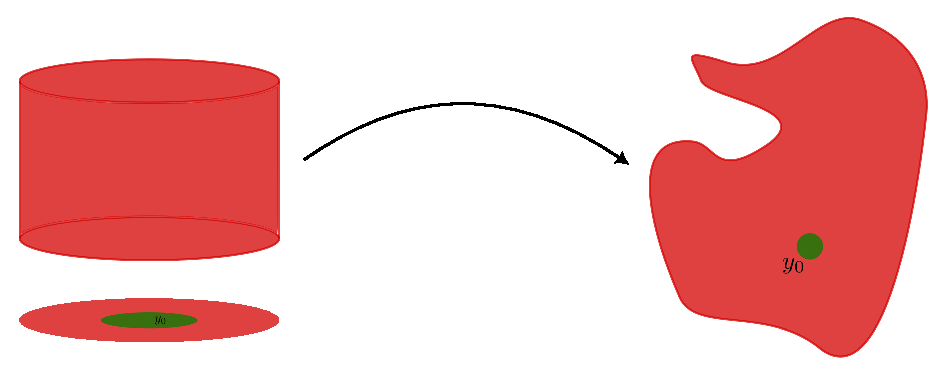
\includegraphics[scale=0.5]{Figures/equiv_homotopy.eps}
        \caption{La definici\'on de $g(x)$ que lleva a un cilindro a un disco
        perforado y rellena el hueco con $y_0$}.
        \label{fig_12}
    \end{figure}
\end{proof}
